\section{Logs}\label{sec:logs}

\lipsum[1]

\clearpage

\subsection{Anàlisi superficial dels \textit{logs}}\label{subsec:log-analysis}

El format dels fitxers d'entrada on hi són emmagatzemats els registres, és d'un text pla on es registren tots els \textit{logs} corresponents a un dia.
Tractant-se de la informació d'accés als recursos d'\gls{UPCommons}, accessibles des de la pàgina web,
tenim aquesta informació recollida des de la capa d'aplicació, mitjançant els missatges de petició del protocol \gls{HTTP}.

\begin{figure}[htbp]
    \centerline{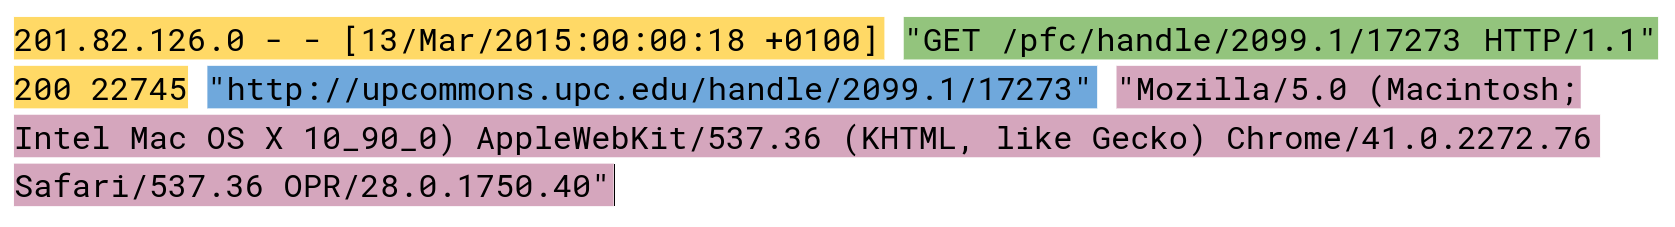
\includegraphics[width=1\textwidth]{figures/example-log}}
    \captionsetup{justification=centering}
    \caption{Exemple del contingut d'un \textit{log}.}\label{fig:example-log}
    \source{UPCommons.}
\end{figure}


\noindent
Cada línia present als fitxers de \textit{logs} correspon a una petició \gls{HTTP} .
El format d'aquest és el següent:

\noindent \\
\textbf{Adreça \gls{IP}} \\ \\
Identificador de xarxa que indica l'agent que ha realitzat la petició.
L'agent pot ser:
\begin{itemize}
    \item Un usuari humà.
    \item Un agent automatitzat: robots, scripts, serveis de mail, etc.
\end{itemize}
Degut a questions de privacitat i protecció de dades, aquest identificador ha sigut modificat en un procés d'anonimització. \\

\begin{tcolorbox}[colback=green!5!white, colframe=green!50!black, title=Els iguals emmascarats]
    No podem sempre afirmar que dues peticions amb el mateix identificador provenen del mateix usuari.
    Pot haver-hi darrere un \gls{NAT}, usuaris compartint dispositiu, etc.
\end{tcolorbox}

\noindent \\
\textbf{Data i hora} \\ \\
La marca temporal del registre ve definida per la seva data i hora.
Si bé es pot treballar directament amb aquest valors si segueix el format \gls{ISO}, és preferible utilitzar el format estàndard \gls{POSIX} (nombre de segons no intercalars des de l'1 de gener del 1970)

\clearpage

\noindent
\textbf{Informació de la petició \gls{HTTP}}~\cite{http} \\

\begin{itemize}
    \item Mètode de la petició: els més habitals són \texttt{GET}, \texttt{POST} i \texttt{HEAD} .
    \item Recurs accedit: enllaç al recurs accedit per la petició.
    \item Versió \gls{HTTP}: evolució d'\texttt{HTTP/1.0} fins a \texttt{HTTP/1.1} en el transcurs dels anys.
    \item Codi d'estat que retorna la petició: codi que representa el resultat de la petició.
    Els més habituals són els \texttt{2XX} (succes), \texttt{4XX} (error del client) i \texttt{5XX} (error del servidor)
    \item Mida de la resposta: mida en \textit{bytes} del cos de la resposta.
\end{itemize}

\noindent \\
\textbf{Referent} \\ \\
El camp del referent indica la ubicació d’on s’ha fet la sol·licitud del recurs accedit.

\noindent \\ \\
\textbf{User Agent} \\ \\
Amb l’ajuda d’aquest camp, podrem analitzar l’empremta digital del cercador utilitzat i determinar amb una certa precisió el tipus de dispositiu utilitzat, el sistema operatiu, si l’acció prové d’un usuari o d’una eina automatitzada (bots o serveis de mail)

\clearpage

\subsection{Filtratge dels \textit{logs}}\label{subsec:log-filter}

Un cop entenem l'estructura dels \textit{logs}, el següent pas és realitzar una anàlisis preliminar del seu contingut.
Esmentarem diferents casos trobats durant el processament d'aquests. \\

\noindent
El cas principal és aquell \textit{log} que incorpori informació sobre un accés a un recurs, o una cerca.
Els podrem identificar perquè:

\begin{itemize}
    \item Porten l’identificador \gls{handle}.
    \item Contenen referències a algun domini d’\gls{UPCommons}.
    \item En cas ser una cerca a la plataforma, porten l’etiqueta amb alguna paraula clau com \textit{discover}, \textit{browse} \dots
\end{itemize}

\noindent
Però els servidors registren \textbf{moltes} més coses.
És feina nostra decidir què fer en cada cas. \\

\noindent
\textbf{Accés a recursos web} \\ \\
Després d’un accés a algun recurs, generalment als \textit{logs} es poden veure registres d’accessos a recursos web (en vermell),
com podrien ser fixters css, javascript, gifs …

\begin{figure}[htbp]
    \centerline{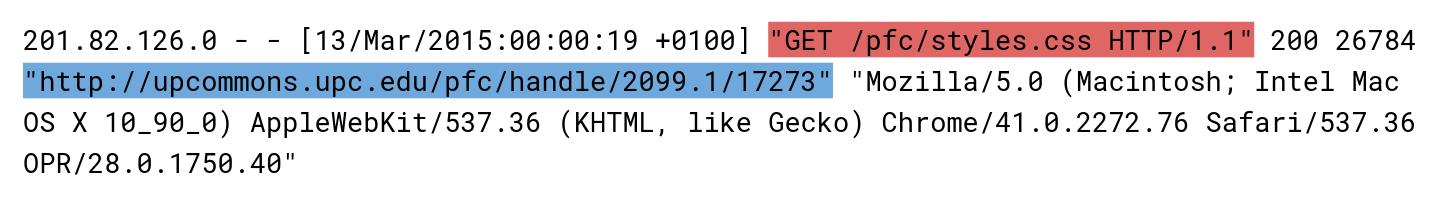
\includegraphics[width=\textwidth]{figures/log-web-resource}}
    \captionsetup{justification=centering}
    \caption{Exemple d'un \textit{log} que accedeix a un recurs web, concretament una fulla d'estils \textit{\gls{CSS}} .}\label{fig:log-web-resource}
    \source{UPCommons.}
\end{figure}

%\begin{figure}[htbp]
%    \centerline{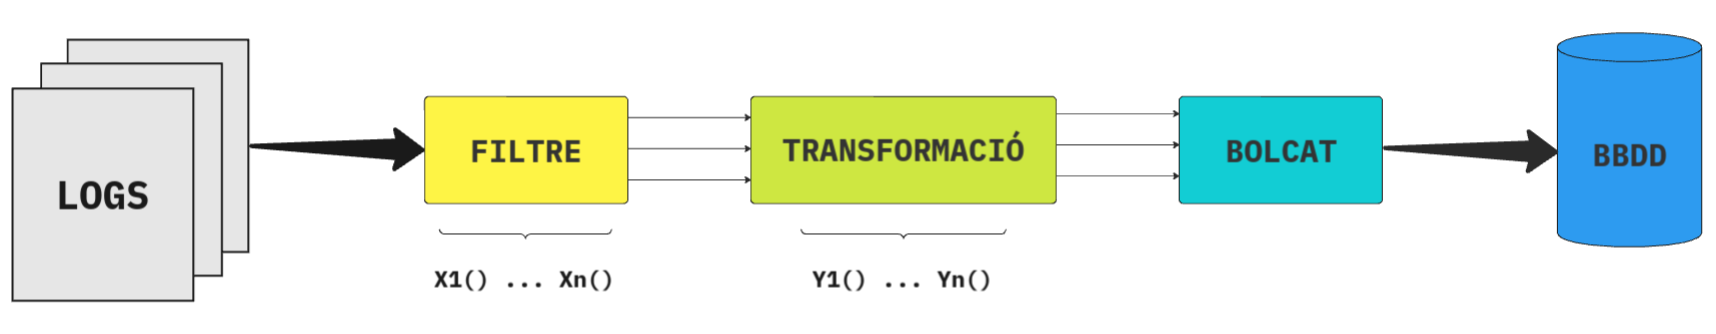
\includegraphics[width=1.3\textwidth]{figures/log-processing}}
%    \captionsetup{justification=centering}
%    \caption{Disseny tècnic del processament dels \textit{logs}.}\label{fig:log-processing}
%    \source{Elaboració pròpia.}
%\end{figure}
%
%\begin{figure}[htbp]
%    \centerline{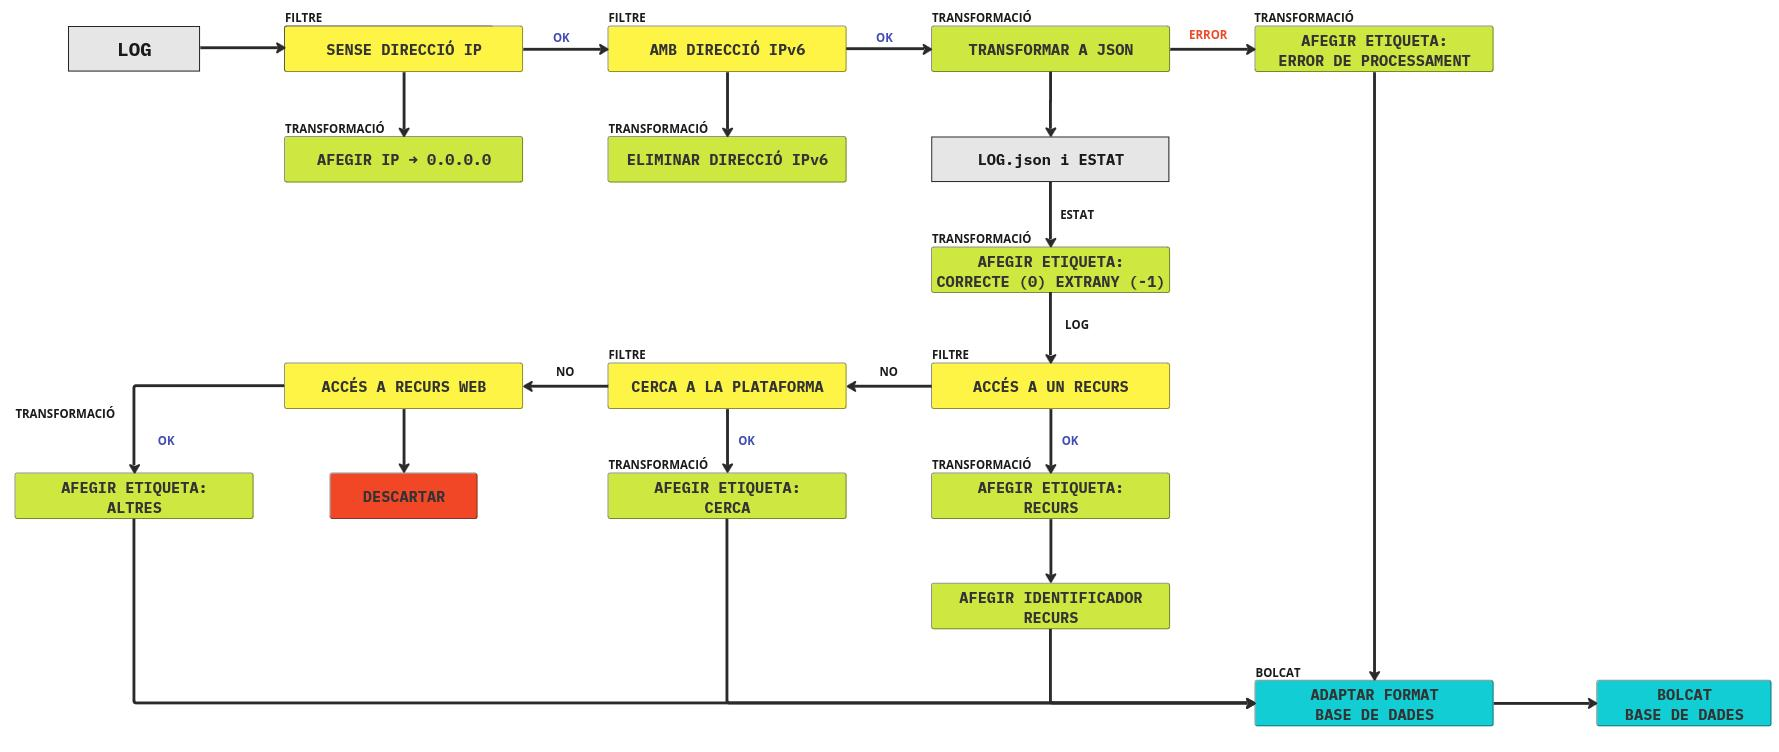
\includegraphics[width=1.5\textwidth]{figures/log-processing-workflow}}
%    \captionsetup{justification=centering}
%    \caption{Implementació del processament dels \textit{logs}.}\label{fig:log-processing-workflow}
%    \source{Elaboració pròpia.}
%\end{figure}
